\subsubsection{Dao động có cản khô}
\begin{frame}{Hệ DĐ có cản khô}
    \begin{center}
        \resizebox{1\linewidth}{!}{


% Pattern Info
 
\tikzset{
pattern size/.store in=\mcSize, 
pattern size = 5pt,
pattern thickness/.store in=\mcThickness, 
pattern thickness = 0.3pt,
pattern radius/.store in=\mcRadius, 
pattern radius = 1pt}
\makeatletter
\pgfutil@ifundefined{pgf@pattern@name@_2kqxtfn0d}{
\pgfdeclarepatternformonly[\mcThickness,\mcSize]{_2kqxtfn0d}
{\pgfqpoint{0pt}{0pt}}
{\pgfpoint{\mcSize+\mcThickness}{\mcSize+\mcThickness}}
{\pgfpoint{\mcSize}{\mcSize}}
{
\pgfsetcolor{\tikz@pattern@color}
\pgfsetlinewidth{\mcThickness}
\pgfpathmoveto{\pgfqpoint{0pt}{0pt}}
\pgfpathlineto{\pgfpoint{\mcSize+\mcThickness}{\mcSize+\mcThickness}}
\pgfusepath{stroke}
}}
\makeatother

% Pattern Info
 
\tikzset{
pattern size/.store in=\mcSize, 
pattern size = 5pt,
pattern thickness/.store in=\mcThickness, 
pattern thickness = 0.3pt,
pattern radius/.store in=\mcRadius, 
pattern radius = 1pt}
\makeatletter
\pgfutil@ifundefined{pgf@pattern@name@_godb81ihg}{
\pgfdeclarepatternformonly[\mcThickness,\mcSize]{_godb81ihg}
{\pgfqpoint{0pt}{0pt}}
{\pgfpoint{\mcSize+\mcThickness}{\mcSize+\mcThickness}}
{\pgfpoint{\mcSize}{\mcSize}}
{
\pgfsetcolor{\tikz@pattern@color}
\pgfsetlinewidth{\mcThickness}
\pgfpathmoveto{\pgfqpoint{0pt}{0pt}}
\pgfpathlineto{\pgfpoint{\mcSize+\mcThickness}{\mcSize+\mcThickness}}
\pgfusepath{stroke}
}}
\makeatother
\tikzset{every picture/.style={line width=0.75pt}} %set default line width to 0.75pt        

\begin{tikzpicture}[x=0.75pt,y=0.75pt,yscale=-1,xscale=1]
%uncomment if require: \path (0,15225); %set diagram left start at 0, and has height of 15225

%Straight Lines [id:da9963445997044897] 
\draw     [color={rgb, 255:red, 0; green, 0; blue, 0 }  ](234.5,1393.22) -- (235,1478.22) ;
%Straight Lines [id:da40001984612577823] 
\draw     [color={rgb, 255:red, 0; green, 0; blue, 0 }  ](460.5,1478.22) -- (235,1478.22) ;
%Shape: Rectangle [id:dp04983777818714219] 
\draw  [draw opacity=0][pattern=_2kqxtfn0d,pattern size=6pt,pattern thickness=0.75pt,pattern radius=0pt, pattern color={rgb, 255:red, 0; green, 0; blue, 0}] (234.5,1393.22) -- (209.5,1393.22) -- (209.5,1478.22) -- (234.5,1478.22) -- cycle ;
%Shape: Resistor [id:dp774135550731575] 
\draw    [color={rgb, 255:red, 0; green, 0; blue, 0 }  ](234.75,1435.72) -- (251.4,1435.72) -- (255.1,1426.84) -- (262.5,1444.59) -- (269.9,1426.84) -- (277.3,1444.59) -- (284.7,1426.84) -- (292.1,1444.59) -- (299.5,1426.84) -- (306.9,1444.59) -- (310.6,1435.72) -- (327.25,1435.72) ;
%Shape: Square [id:dp21336352659463942] 
\draw    [color={rgb, 255:red, 0; green, 0; blue, 0 }  ](327.5,1393.22) -- (412.5,1393.22) -- (412.5,1478.22) -- (327.5,1478.22) -- cycle ;
%Straight Lines [id:da7073291864375937] 
\draw     [color={rgb, 255:red, 0; green, 0; blue, 0 }  ](479.5,1512.21) -- (399.5,1512) ;
\draw [shift={(399.5,1512)}, rotate = 0.15] [color={rgb, 255:red, 0; green, 0; blue, 0 }  ][line width=0.75]    (0,5.59) -- (0,-5.59)   ;
\draw [shift={(482.5,1512.22)}, rotate = 180.15] [fill={rgb, 255:red, 0; green, 0; blue, 0 }  ][line width=0.08]  [draw opacity=0] (8.93,-4.29) -- (0,0) -- (8.93,4.29) -- cycle    ;
%Straight Lines [id:da9430597363414568] 
\draw     [color={rgb, 255:red, 0; green, 0; blue, 0 }  ](399.5,1512) -- (263.5,1512.22) ;
%Straight Lines [id:da42637684130339726] 
\draw [color={rgb, 255:red, 58; green, 113; blue, 176 }  ,draw opacity=1 ][line width=2.25]    (327.5,1476.22) -- (275.5,1476.22) ;
\draw [shift={(270.5,1476.22)}, rotate = 360] [fill={rgb, 255:red, 58; green, 113; blue, 176 }  ,fill opacity=1 ][line width=0.08]  [draw opacity=0] (14.29,-6.86) -- (0,0) -- (14.29,6.86) -- cycle    ;
%Straight Lines [id:da9325818154663401] 
\draw     [color={rgb, 255:red, 0; green, 0; blue, 0 }  ](595.5,1393.22) -- (596,1478.22) ;
%Straight Lines [id:da28331355274785697] 
\draw     [color={rgb, 255:red, 0; green, 0; blue, 0 }  ](821.5,1478.22) -- (596,1478.22) ;
%Shape: Rectangle [id:dp8766070931807493] 
\draw  [draw opacity=0][pattern=_godb81ihg,pattern size=6pt,pattern thickness=0.75pt,pattern radius=0pt, pattern color={rgb, 255:red, 0; green, 0; blue, 0}] (595.5,1393.22) -- (570.5,1393.22) -- (570.5,1478.22) -- (595.5,1478.22) -- cycle ;
%Shape: Resistor [id:dp449600202945972] 
\draw    [color={rgb, 255:red, 0; green, 0; blue, 0 }  ](595.75,1435.72) -- (612.4,1435.72) -- (616.1,1426.84) -- (623.5,1444.59) -- (630.9,1426.84) -- (638.3,1444.59) -- (645.7,1426.84) -- (653.1,1444.59) -- (660.5,1426.84) -- (667.9,1444.59) -- (671.6,1435.72) -- (688.25,1435.72) ;
%Shape: Square [id:dp9555174596265368] 
\draw   [color={rgb, 255:red, 0; green, 0; blue, 0 }  ](688.5,1393.22) -- (773.5,1393.22) -- (773.5,1478.22) -- (688.5,1478.22) -- cycle ;
%Straight Lines [id:da6819265028764014] 
\draw [color={rgb, 255:red, 0; green, 0; blue, 0 }  ](840.5,1512.21) -- (760.5,1512) ;
\draw [shift={(760.5,1512)}, rotate = 0.15] [color={rgb, 255:red, 0; green, 0; blue, 0 }  ][line width=0.75]    (0,5.59) -- (0,-5.59)   ;
\draw [shift={(843.5,1512.22)}, rotate = 180.15] [fill={rgb, 255:red, 0; green, 0; blue, 0 }  ][line width=0.08]  [draw opacity=0] (8.93,-4.29) -- (0,0) -- (8.93,4.29) -- cycle    ;
%Straight Lines [id:da6949123016758587] 
\draw    [color={rgb, 255:red, 0; green, 0; blue, 0 }  ](760.5,1512) -- (624.5,1512.22) ;
%Straight Lines [id:da5194904336424693] 
\draw [color={rgb, 255:red, 58; green, 113; blue, 176 }  ,draw opacity=1 ][line width=2.25]    (773.5,1476.22) -- (828.5,1476.22) ;
\draw [shift={(833.5,1476.22)}, rotate = 180] [fill={rgb, 255:red, 58; green, 113; blue, 176 }  ,fill opacity=1 ][line width=0.08]  [draw opacity=0] (14.29,-6.86) -- (0,0) -- (14.29,6.86) -- cycle    ;
%Straight Lines [id:da27717182588678657] 
\draw [color={wsdred}  ,draw opacity=1 ][line width=1.5]    (412,1434.5) -- (433.5,1434.5) ;
\draw [shift={(437.5,1434.5)}, rotate = 180] [fill={wsdred}  ,fill opacity=1 ][line width=0.08]  [draw opacity=0] (11.61,-5.58) -- (0,0) -- (11.61,5.58) -- cycle    ;
%Straight Lines [id:da17073897628277557] 
\draw [color={wsdred}  ,draw opacity=1 ][line width=1.5]    (689,1436.5) -- (665.5,1436.5) ;
\draw [shift={(661.5,1436.5)}, rotate = 360] [fill={wsdred}  ,fill opacity=1 ][line width=0.08]  [draw opacity=0] (11.61,-5.58) -- (0,0) -- (11.61,5.58) -- cycle    ;

% Text Node
\draw (276,1401.22) node [anchor=north west][inner sep=0.75pt]   [align=left] {\textcolor{black}{k}};
% Text Node
\draw (482.5,1512.22) node [anchor=north west][inner sep=0.75pt]   [align=left] {\textcolor{black}{$x$}};
% Text Node
\draw (370,1435.72) node   [align=left] {\textcolor{black}{m}};
% Text Node
\draw (399.5,1519) node [anchor=north] [inner sep=0.75pt]   [align=left] {\textcolor{black}{$O$}};
% Text Node
\draw (214,1485) node [anchor=north west][inner sep=0.75pt]  [color={rgb, 255:red, 58; green, 113; blue, 176 }  ,opacity=1 ]  {$|\vec{F}_{1} |\ =\mu \ N\ $};
% Text Node
\draw (637,1401.22) node [anchor=north west][inner sep=0.75pt]   [align=left] {\textcolor{black}{k}};
% Text Node
\draw (843.5,1512.22) node [anchor=north west][inner sep=0.75pt]   [align=left] {\textcolor{black}{$x$}};
% Text Node
\draw (731,1435.72) node   [align=left] {\textcolor{black}{m}};
% Text Node
\draw (760.5,1519) node [anchor=north] [inner sep=0.75pt]   [align=left] {\textcolor{black}{$O$}};
% Text Node
\draw (773.5,1485) node [anchor=north west][inner sep=0.75pt]  [color={rgb, 255:red, 58; green, 113; blue, 176 }  ,opacity=1 ]  {$|\vec{F}_{1} |\ =\mu \ N\ $};
% Text Node
\draw (418,1405.5) node [anchor=north west][inner sep=0.75pt]  [color={wsdred}  ,opacity=1 ]  {$\vec{v}$};
% Text Node
\draw (669,1405.5) node [anchor=north west][inner sep=0.75pt]  [color={wsdred}  ,opacity=1 ]  {$\vec{v}$};


% Text Node
\draw (214,1550) node [anchor=north west][inner sep=0.75pt]  [color={wsdred}  ,opacity=1 ]  {\large (A)};
% Text Node
\draw (580,1550) node [anchor=north west][inner sep=0.75pt]  [color={wsdred}  ,opacity=1 ]  {\large (B)};

\end{tikzpicture}

}
    \end{center}
    Lúc này hệ chịu thêm một lực ma sát khô. Tổng lực tác động lên vật

\end{frame}
\begin{frame}{Hệ DĐ có cản khô - PTVP}
    Lúc này ta giải cùng lúc hai phương trình vi phân
    \begin{equation}
    \left\{
        \begin{split}
            m x'' &= -kx + \mu N \\
            m x'' &= -kx - \mu N
        \end{split}
    \right.
    \label{eq:2.2_1}
    \end{equation}
    Đặt \(a=x-\mu N/k\) và \(b=x+\mu N/k\) ta có.
    \begin{equation}
    \left\{
        \begin{split}
        a'' + \omega^2 a &= 0 \\
        b'' + \omega^2 b &= 0
        \end{split}
    \right.
    \label{2.2_2}
    \end{equation}
    Ta có hai nghiệm:
    \begin{equation}
    \left\{
        \begin{array}{ccc}
        a &=&\displaystyle x -\frac{\mu N}{k} = A \cos{(\omega t + \varphi_a)} 
        \\
        \\
        b &=&\displaystyle x +\frac{\mu N}{k} = B \cos{(\omega t + \varphi_b)}
        \end{array}
    \right.
    \label{eq:2.2_3}
    \end{equation}
\end{frame}

\begin{frame}{Hệ DĐ có cản khô - PTVP}
    Nghiệm \(a\) ứng với trường hợp vật đang đi cùng chiều dương. Nghiệm \(b\) ứng với trường hợp vật đang đi ngược chiều dương. 
    \vspace{2mm}

    Trường hợp vật đi giống nghiệm \(a\)
    \vspace{5mm}
    
    \begin{center}
        


% Pattern Info
 
\tikzset{
pattern size/.store in=\mcSize, 
pattern size = 5pt,
pattern thickness/.store in=\mcThickness, 
pattern thickness = 0.3pt,
pattern radius/.store in=\mcRadius, 
pattern radius = 1pt}
\makeatletter
\pgfutil@ifundefined{pgf@pattern@name@_lh2po6njo}{
\pgfdeclarepatternformonly[\mcThickness,\mcSize]{_lh2po6njo}
{\pgfqpoint{0pt}{0pt}}
{\pgfpoint{\mcSize+\mcThickness}{\mcSize+\mcThickness}}
{\pgfpoint{\mcSize}{\mcSize}}
{
\pgfsetcolor{\tikz@pattern@color}
\pgfsetlinewidth{\mcThickness}
\pgfpathmoveto{\pgfqpoint{0pt}{0pt}}
\pgfpathlineto{\pgfpoint{\mcSize+\mcThickness}{\mcSize+\mcThickness}}
\pgfusepath{stroke}
}}
\makeatother
\tikzset{every picture/.style={line width=0.75pt}} %set default line width to 0.75pt        

\begin{tikzpicture}[x=0.75pt,y=0.75pt,yscale=-1,xscale=1]
%uncomment if require: \path (0,15225); %set diagram left start at 0, and has height of 15225

%Straight Lines [id:da6176525847406964] 
\draw  [color={rgb, 255:red, 0; green, 0; blue, 0 }  ]  (81,1232) -- (81,1264) ;
%Straight Lines [id:da9199900839912454] 
\draw  [color={rgb, 255:red, 0; green, 0; blue, 0 }  ]  (410.5,1264) -- (81,1264) ;
%Shape: Rectangle [id:dp7184973668577894] 
\draw  [draw opacity=0][pattern=_lh2po6njo,pattern size=6pt,pattern thickness=0.75pt,pattern radius=0pt, pattern color={rgb, 255:red, 0; green, 0; blue, 0}] (81,1232) -- (55.5,1232) -- (55.5,1264) -- (81,1264) -- cycle ;
%Shape: Resistor [id:dp21078579575471013] 
\draw [color={rgb, 255:red, 0; green, 0; blue, 0 }  ]  (81,1248) -- (97.65,1248) -- (101.35,1239.13) -- (108.75,1256.88) -- (116.15,1239.13) -- (123.55,1256.88) -- (130.95,1239.13) -- (138.35,1256.88) -- (145.75,1239.13) -- (153.15,1256.88) -- (156.85,1248) -- (173.5,1248) ;
%Shape: Square [id:dp9600989184404278] 
\draw [color={rgb, 255:red, 0; green, 0; blue, 0 }  ]  (173.5,1232) -- (205.5,1232) -- (205.5,1264) -- (173.5,1264) -- cycle ;
%Straight Lines [id:da40932176761609584] 
\draw [color={rgb, 255:red, 0; green, 0; blue, 0 }  ]   (283.5,1308) -- (400.5,1308) ;
\draw [shift={(402.5,1308)}, rotate = 180] [color={rgb, 255:red, 0; green, 0; blue, 0 }  ][line width=0.75]    (10.93,-3.29) .. controls (6.95,-1.4) and (3.31,-0.3) .. (0,0) .. controls (3.31,0.3) and (6.95,1.4) .. (10.93,3.29)   ;
%Straight Lines [id:da22152521277286796] 
\draw [color={rgb, 255:red, 0; green, 0; blue, 0 }  ]   (189.5,1308) -- (283.5,1308) ;
\draw [shift={(283.5,1308)}, rotate = 180] [color={rgb, 255:red, 0; green, 0; blue, 0 }  ][line width=0.75]    (0,5.59) -- (0,-5.59)   ;
%Straight Lines [id:da7786268386075514] 
\draw [color={rgb, 255:red, 0; green, 0; blue, 0 }  ]   (134,1308) -- (189.5,1308) ;
\draw [shift={(189.5,1308)}, rotate = 180] [color={rgb, 255:red, 0; green, 0; blue, 0 }  ][line width=0.75]    (0,5.59) -- (0,-5.59)   ;
%Straight Lines [id:da7785698063711466] 
\draw [color={rgb, 255:red, 0; green, 0; blue, 0 }  ]   (189.5,1308) -- (250.5,1308) ;
\draw [shift={(250.5,1308)}, rotate = 180] [color={rgb, 255:red, 0; green, 0; blue, 0 }  ][line width=0.75]    (0,5.59) -- (0,-5.59)   ;
%Straight Lines [id:da3083733910153268] 
\draw [color={rgb, 255:red, 0; green, 0; blue, 0 }  ]   (250.5,1308) -- (311.5,1308) ;
\draw [shift={(311.5,1308)}, rotate = 180] [color={rgb, 255:red, 0; green, 0; blue, 0 }  ][line width=0.75]    (0,5.59) -- (0,-5.59)   ;

% Text Node
\draw (189.5,1248) node   [align=left] {\textcolor{black}{m}};
% Text Node
\draw (275,1279) node [anchor=north west][inner sep=0.75pt]    {\textcolor{black}{$O$}};
% Text Node
\draw (181,1323) node [anchor=north west][inner sep=0.75pt]    {\textcolor{black}{$A_0$}};
% Text Node
\draw (241,1323) node [anchor=north west][inner sep=0.75pt]    {\textcolor{black}{$O'$}};
% Text Node
\draw (302,1323) node [anchor=north west][inner sep=0.75pt]    {\textcolor{black}{$A_1$}};


\end{tikzpicture}
    \end{center}
\end{frame}
\begin{frame}{Hệ DĐ có cản khô - PTVP}
    Trường hợp vật đi giống nghiệm \(b\)
    \vspace{5mm}
    
    \begin{center}
        


% Pattern Info
 
\tikzset{
pattern size/.store in=\mcSize, 
pattern size = 5pt,
pattern thickness/.store in=\mcThickness, 
pattern thickness = 0.3pt,
pattern radius/.store in=\mcRadius, 
pattern radius = 1pt}
\makeatletter
\pgfutil@ifundefined{pgf@pattern@name@_lh7bvwhj0}{
\pgfdeclarepatternformonly[\mcThickness,\mcSize]{_lh7bvwhj0}
{\pgfqpoint{0pt}{0pt}}
{\pgfpoint{\mcSize+\mcThickness}{\mcSize+\mcThickness}}
{\pgfpoint{\mcSize}{\mcSize}}
{
\pgfsetcolor{\tikz@pattern@color}
\pgfsetlinewidth{\mcThickness}
\pgfpathmoveto{\pgfqpoint{0pt}{0pt}}
\pgfpathlineto{\pgfpoint{\mcSize+\mcThickness}{\mcSize+\mcThickness}}
\pgfusepath{stroke}
}}
\makeatother
\tikzset{every picture/.style={line width=0.75pt}} %set default line width to 0.75pt        

\begin{tikzpicture}[x=0.75pt,y=0.75pt,yscale=-1,xscale=1]
%uncomment if require: \path (0,15225); %set diagram left start at 0, and has height of 15225

%Straight Lines [id:da6176525847406964] 
\draw [color={rgb, 255:red, 0; green, 0; blue, 0 }  ,draw opacity=1 ]   (81,1232) -- (81,1264) ;
%Straight Lines [id:da9199900839912454] 
\draw [color={rgb, 255:red, 0; green, 0; blue, 0 }  ,draw opacity=1 ]   (410.5,1264) -- (81,1264) ;
%Shape: Rectangle [id:dp7184973668577894] 
\draw  [draw opacity=0][pattern=_lh7bvwhj0,pattern size=6pt,pattern thickness=0.75pt,pattern radius=0pt, pattern color={rgb, 255:red, 0; green, 0; blue, 0}] (81,1232) -- (55.5,1232) -- (55.5,1264) -- (81,1264) -- cycle ;
%Shape: Square [id:dp9600989184404278] 
\draw  [color={rgb, 255:red, 0; green, 0; blue, 0 }  ,draw opacity=1 ] (324.5,1232) -- (356.5,1232) -- (356.5,1264) -- (324.5,1264) -- cycle ;
%Straight Lines [id:da40932176761609584] 
\draw [color={rgb, 255:red, 0; green, 0; blue, 0 }  ,draw opacity=1 ]   (283.5,1308) -- (400.5,1308) ;
\draw [shift={(402.5,1308)}, rotate = 180] [color={rgb, 255:red, 0; green, 0; blue, 0 }  ,draw opacity=1 ][line width=0.75]    (10.93,-3.29) .. controls (6.95,-1.4) and (3.31,-0.3) .. (0,0) .. controls (3.31,0.3) and (6.95,1.4) .. (10.93,3.29)   ;
%Straight Lines [id:da7786268386075514] 
\draw [color={rgb, 255:red, 0; green, 0; blue, 0 }  ,draw opacity=1 ]   (134,1308) -- (189.5,1308) ;
%Straight Lines [id:da7785698063711466] 
\draw [color={rgb, 255:red, 0; green, 0; blue, 0 }  ,draw opacity=1 ]   (189.5,1308) -- (250.5,1308) ;
\draw [shift={(250.5,1308)}, rotate = 180] [color={rgb, 255:red, 0; green, 0; blue, 0 }  ,draw opacity=1 ][line width=0.75]    (0,5.59) -- (0,-5.59)   ;
%Straight Lines [id:da3083733910153268] 
\draw [color={rgb, 255:red, 0; green, 0; blue, 0 }  ,draw opacity=1 ]   (283.5,1308) -- (343,1308) ;
\draw [shift={(343,1308)}, rotate = 180] [color={rgb, 255:red, 0; green, 0; blue, 0 }  ,draw opacity=1 ][line width=0.75]    (0,5.59) -- (0,-5.59)   ;
%Shape: Resistor [id:dp7960558718882587] 
\draw  [color={rgb, 255:red, 0; green, 0; blue, 0 }  ,draw opacity=1 ] (81,1248) -- (124.65,1248) -- (134.35,1237.33) -- (153.75,1258.67) -- (173.15,1237.33) -- (192.55,1258.67) -- (211.95,1237.33) -- (231.35,1258.67) -- (250.75,1237.33) -- (270.15,1258.67) -- (279.85,1248) -- (323.5,1248) ;
%Straight Lines [id:da35230297648233777] 
\draw [color={rgb, 255:red, 0; green, 0; blue, 0 }  ,draw opacity=1 ]   (250.5,1308) -- (283.5,1308) ;
\draw [shift={(283.5,1308)}, rotate = 180] [color={rgb, 255:red, 0; green, 0; blue, 0 }  ,draw opacity=1 ][line width=0.75]    (0,5.59) -- (0,-5.59)   ;
%Straight Lines [id:da9955873343145762] 
\draw [color={rgb, 255:red, 0; green, 0; blue, 0 }  ,draw opacity=1 ]   (224,1308) -- (283.5,1308) ;
\draw [shift={(224,1308)}, rotate = 180] [color={rgb, 255:red, 0; green, 0; blue, 0 }  ,draw opacity=1 ][line width=0.75]    (0,5.59) -- (0,-5.59)   ;

% Text Node
\draw (340.5,1248) node   [align=left] {m};
% Text Node
\draw (272,1321) node [anchor=north west][inner sep=0.75pt]    {$O'$};
% Text Node
\draw (214,1320) node [anchor=north west][inner sep=0.75pt]    {$A_{1}$};
% Text Node
\draw (242,1276) node [anchor=north west][inner sep=0.75pt]    {$O$};
% Text Node
\draw (334,1321) node [anchor=north west][inner sep=0.75pt]    {$A_{0}$};


\end{tikzpicture}

    \end{center}
    Trong một chu kỳ, vật tham gia lần lượt cả hai quy luật chuyển động. Lấy ví dụ sau.

\end{frame}
\begin{frame}{Hệ DĐ có cản khô - Biên độ}
    \begin{center}
        \scalebox{0.6}{


\tikzset{every picture/.style={line width=0.75pt}} %set default line width to 0.75pt        

\begin{tikzpicture}[x=0.75pt,y=0.75pt,yscale=-1,xscale=1]
%uncomment if require: \path (0,15225); %set diagram left start at 0, and has height of 15225

%Straight Lines [id:da8440235981456923] 
\draw [color={rgb, 255:red, 0; green, 0; blue, 0 }  ,draw opacity=1 ]   (748.5,4556) -- (112.5,4556) ;
%Shape: Square [id:dp7730743948956422] 
\draw  [color={rgb, 255:red, 0; green, 0; blue, 0 }  ,draw opacity=1 ] (229.5,4524) -- (261.5,4524) -- (261.5,4556) -- (229.5,4556) -- cycle ;
%Straight Lines [id:da5849410238032737] 
\draw [color={rgb, 255:red, 0; green, 0; blue, 0 }  ,draw opacity=1 ][line width=1.5]    (433.5,4600) -- (747.5,4600) ;
\draw [shift={(750.5,4600)}, rotate = 180] [color={rgb, 255:red, 0; green, 0; blue, 0 }  ,draw opacity=1 ][line width=1.5]    (14.21,-4.28) .. controls (9.04,-1.82) and (4.3,-0.39) .. (0,0) .. controls (4.3,0.39) and (9.04,1.82) .. (14.21,4.28)   ;
%Straight Lines [id:da501337374602] 
\draw [color={rgb, 255:red, 0; green, 0; blue, 0 }  ,draw opacity=1 ][line width=1.5]    (245.5,4600) -- (433.5,4600) ;
\draw [shift={(433.5,4600)}, rotate = 180] [color={rgb, 255:red, 0; green, 0; blue, 0 }  ,draw opacity=1 ][line width=1.5]    (0,6.71) -- (0,-6.71)   ;
%Straight Lines [id:da8338549647082345] 
\draw [color={rgb, 255:red, 0; green, 0; blue, 0 }  ,draw opacity=1 ][line width=1.5]    (112.5,4600) -- (245.5,4600) ;
\draw [shift={(245.5,4600)}, rotate = 180] [color={rgb, 255:red, 0; green, 0; blue, 0 }  ,draw opacity=1 ][line width=1.5]    (0,6.71) -- (0,-6.71)   ;
%Straight Lines [id:da5472639759035778] 
\draw [color={rgb, 255:red, 0; green, 0; blue, 0 }  ,draw opacity=1 ]   (748.5,4694) -- (112.5,4694) ;
%Shape: Square [id:dp11345606497116645] 
\draw  [color={rgb, 255:red, 0; green, 0; blue, 0 }  ,draw opacity=1 ] (544.5,4662) -- (576.5,4662) -- (576.5,4694) -- (544.5,4694) -- cycle ;
%Straight Lines [id:da28185616117474566] 
\draw [color={rgb, 255:red, 0; green, 0; blue, 0 }  ,draw opacity=1 ][line width=1.5]    (433.5,4738) -- (747.5,4738) ;
\draw [shift={(750.5,4738)}, rotate = 180] [color={rgb, 255:red, 0; green, 0; blue, 0 }  ,draw opacity=1 ][line width=1.5]    (14.21,-4.28) .. controls (9.04,-1.82) and (4.3,-0.39) .. (0,0) .. controls (4.3,0.39) and (9.04,1.82) .. (14.21,4.28)   ;
%Straight Lines [id:da614812825007393] 
\draw [color={rgb, 255:red, 0; green, 0; blue, 0 }  ,draw opacity=1 ][line width=1.5]    (245.5,4738) -- (433.5,4738) ;
\draw [shift={(433.5,4738)}, rotate = 180] [color={rgb, 255:red, 0; green, 0; blue, 0 }  ,draw opacity=1 ][line width=1.5]    (0,6.71) -- (0,-6.71)   ;
%Straight Lines [id:da3151466941990222] 
\draw [color={rgb, 255:red, 0; green, 0; blue, 0 }  ,draw opacity=1 ][line width=1.5]    (112.5,4738) -- (245.5,4738) ;
\draw [shift={(245.5,4738)}, rotate = 180] [color={rgb, 255:red, 0; green, 0; blue, 0 }  ,draw opacity=1 ][line width=1.5]    (0,6.71) -- (0,-6.71)   ;
%Straight Lines [id:da16801387670839896] 
\draw [color={rgb, 255:red, 0; green, 0; blue, 0 }  ,draw opacity=1 ][line width=1.5]    (433.5,4738) -- (561.5,4738) ;
\draw [shift={(561.5,4738)}, rotate = 180] [color={rgb, 255:red, 0; green, 0; blue, 0 }  ,draw opacity=1 ][line width=1.5]    (0,6.71) -- (0,-6.71)   ;
%Straight Lines [id:da7824565205771314] 
\draw [color={rgb, 255:red, 0; green, 0; blue, 0 }  ,draw opacity=1 ]   (749.5,4834) -- (113.5,4834) ;
%Shape: Square [id:dp10726696816762793] 
\draw  [color={rgb, 255:red, 0; green, 0; blue, 0 }  ,draw opacity=1 ] (339.5,4802) -- (371.5,4802) -- (371.5,4834) -- (339.5,4834) -- cycle ;
%Straight Lines [id:da5556513504225804] 
\draw [color={rgb, 255:red, 0; green, 0; blue, 0 }  ,draw opacity=1 ][line width=1.5]    (434.5,4878) -- (748.5,4878) ;
\draw [shift={(751.5,4878)}, rotate = 180] [color={rgb, 255:red, 0; green, 0; blue, 0 }  ,draw opacity=1 ][line width=1.5]    (14.21,-4.28) .. controls (9.04,-1.82) and (4.3,-0.39) .. (0,0) .. controls (4.3,0.39) and (9.04,1.82) .. (14.21,4.28)   ;
%Straight Lines [id:da35868213260288484] 
\draw [color={rgb, 255:red, 0; green, 0; blue, 0 }  ,draw opacity=1 ][line width=1.5]    (246.5,4878) -- (434.5,4878) ;
\draw [shift={(434.5,4878)}, rotate = 180] [color={rgb, 255:red, 0; green, 0; blue, 0 }  ,draw opacity=1 ][line width=1.5]    (0,6.71) -- (0,-6.71)   ;
%Straight Lines [id:da9226047069569581] 
\draw [color={rgb, 255:red, 0; green, 0; blue, 0 }  ,draw opacity=1 ][line width=1.5]    (113.5,4878) -- (246.5,4878) ;
\draw [shift={(246.5,4878)}, rotate = 180] [color={rgb, 255:red, 0; green, 0; blue, 0 }  ,draw opacity=1 ][line width=1.5]    (0,6.71) -- (0,-6.71)   ;
%Straight Lines [id:da39824710137073915] 
\draw [color={rgb, 255:red, 0; green, 0; blue, 0 }  ,draw opacity=1 ][line width=1.5]    (434.5,4878) -- (562.5,4878) ;
\draw [shift={(562.5,4878)}, rotate = 180] [color={rgb, 255:red, 0; green, 0; blue, 0 }  ,draw opacity=1 ][line width=1.5]    (0,6.71) -- (0,-6.71)   ;
%Straight Lines [id:da5711245809745336] 
\draw [color={rgb, 255:red, 0; green, 0; blue, 0 }  ,draw opacity=1 ][line width=1.5]    (357.5,4878) -- (434.5,4878) ;
\draw [shift={(357.5,4878)}, rotate = 180] [color={rgb, 255:red, 0; green, 0; blue, 0 }  ,draw opacity=1 ][line width=1.5]    (0,6.71) -- (0,-6.71)   ;
%Straight Lines [id:da2785554999977735] 
\draw [color={rgb, 255:red, 0; green, 0; blue, 0 }  ,draw opacity=1 ] [dash pattern={on 0.84pt off 2.51pt}]  (274,4538) -- (541.5,4538) ;
\draw [shift={(543.5,4538)}, rotate = 180] [color={rgb, 255:red, 0; green, 0; blue, 0 }  ,draw opacity=1 ][line width=0.75]    (10.93,-3.29) .. controls (6.95,-1.4) and (3.31,-0.3) .. (0,0) .. controls (3.31,0.3) and (6.95,1.4) .. (10.93,3.29)   ;
%Straight Lines [id:da5363770674501016] 
\draw [color={rgb, 255:red, 0; green, 0; blue, 0 }  ,draw opacity=1 ] [dash pattern={on 0.84pt off 2.51pt}]  (384.5,4677) -- (536.5,4677) ;
\draw [shift={(382.5,4677)}, rotate = 0] [color={rgb, 255:red, 0; green, 0; blue, 0 }  ,draw opacity=1 ][line width=0.75]    (10.93,-3.29) .. controls (6.95,-1.4) and (3.31,-0.3) .. (0,0) .. controls (3.31,0.3) and (6.95,1.4) .. (10.93,3.29)   ;
%Curve Lines [id:da8774718138615303] 
\draw [color={rgb, 255:red, 0; green, 0; blue, 0 }  ,draw opacity=1 ]   (807,4555) .. controls (842.32,4565.95) and (875.17,4657.08) .. (803.59,4693.46) ;
\draw [shift={(802.5,4694)}, rotate = 333.75] [color={rgb, 255:red, 0; green, 0; blue, 0 }  ,draw opacity=1 ][line width=0.75]    (10.93,-3.29) .. controls (6.95,-1.4) and (3.31,-0.3) .. (0,0) .. controls (3.31,0.3) and (6.95,1.4) .. (10.93,3.29)   ;
%Curve Lines [id:da6809827298064757] 
\draw [color={rgb, 255:red, 0; green, 0; blue, 0 }  ,draw opacity=1 ]   (812,4702) .. controls (847.32,4712.95) and (880.17,4804.08) .. (808.59,4840.46) ;
\draw [shift={(807.5,4841)}, rotate = 333.75] [color={rgb, 255:red, 0; green, 0; blue, 0 }  ,draw opacity=1 ][line width=0.75]    (10.93,-3.29) .. controls (6.95,-1.4) and (3.31,-0.3) .. (0,0) .. controls (3.31,0.3) and (6.95,1.4) .. (10.93,3.29)   ;

% Text Node
\draw (245.5,4540) node   [align=left] {\textcolor{black}{m}};
% Text Node
\draw (424,4613) node [anchor=north west][inner sep=0.75pt]    {\textcolor{black}{$O$}};
% Text Node
\draw (238,4609) node [anchor=north west][inner sep=0.75pt]    {\textcolor{black}{$A_{0}$}};
% Text Node
\draw (560.5,4678) node   [align=left] {\textcolor{black}{m}};
% Text Node
\draw (424,4751) node [anchor=north west][inner sep=0.75pt]    {\textcolor{black}{$O$}};
% Text Node
\draw (238,4747) node [anchor=north west][inner sep=0.75pt]    {\textcolor{black}{$A_{0}$}};
% Text Node
\draw (549,4747) node [anchor=north west][inner sep=0.75pt]    {\textcolor{black}{$A_{1}$}};
% Text Node
\draw (355.5,4818) node   [align=left] {\textcolor{black}{m}};
% Text Node
\draw (425,4891) node [anchor=north west][inner sep=0.75pt]    {\textcolor{black}{$O$}};
% Text Node
\draw (239,4887) node [anchor=north west][inner sep=0.75pt]    {\textcolor{black}{$A_{0}$}};
% Text Node
\draw (550,4888) node [anchor=north west][inner sep=0.75pt]    {\textcolor{black}{$A_{1}$}};
% Text Node
\draw (345,4887) node [anchor=north west][inner sep=0.75pt]    {\textcolor{black}{$A_{2}$}};
% Text Node
\draw (861,4615) node [anchor=north west][inner sep=0.75pt]    {\textcolor{black}{$T/2$}};
% Text Node
\draw (866,4762) node [anchor=north west][inner sep=0.75pt]    {\textcolor{black}{$T/2$}};
% Text Node
\draw (66,4534) node [anchor=north west][inner sep=0.75pt]   [align=left] {(A)};
% Text Node
\draw (69,4674) node [anchor=north west][inner sep=0.75pt]   [align=left] {(B)};
% Text Node
\draw (70,4812) node [anchor=north west][inner sep=0.75pt]   [align=left] {(C)};


\end{tikzpicture}}
    \end{center}
\end{frame}
\begin{frame}{Hệ DĐ có cản khô - Biên độ}
    Công thức liên hệ giữa hai biên độ liên tiếp là 
    \begin{equation}
        A_{k+1} = A_k - 2 \mu mg/k
        \label{eq:2.2_4}
    \end{equation}
\end{frame}
\subsubsection{Dao động có cản nhớt}
\begin{frame}{Hệ DĐ có cản nhớt}
    \begin{center}
        \resizebox{0.6\linewidth}{!}{


% Pattern Info
 
\tikzset{
pattern size/.store in=\mcSize, 
pattern size = 5pt,
pattern thickness/.store in=\mcThickness, 
pattern thickness = 0.3pt,
pattern radius/.store in=\mcRadius, 
pattern radius = 1pt}
\makeatletter
\pgfutil@ifundefined{pgf@pattern@name@_hkp691r1q}{
\pgfdeclarepatternformonly[\mcThickness,\mcSize]{_hkp691r1q}
{\pgfqpoint{0pt}{0pt}}
{\pgfpoint{\mcSize+\mcThickness}{\mcSize+\mcThickness}}
{\pgfpoint{\mcSize}{\mcSize}}
{
\pgfsetcolor{\tikz@pattern@color}
\pgfsetlinewidth{\mcThickness}
\pgfpathmoveto{\pgfqpoint{0pt}{0pt}}
\pgfpathlineto{\pgfpoint{\mcSize+\mcThickness}{\mcSize+\mcThickness}}
\pgfusepath{stroke}
}}
\makeatother
\tikzset{every picture/.style={line width=0.75pt}} %set default line width to 0.75pt        

\begin{tikzpicture}[x=0.75pt,y=0.75pt,yscale=-1,xscale=1]
%uncomment if require: \path (0,15225); %set diagram left start at 0, and has height of 15225

%Straight Lines [id:da37304025889826953] 
\draw [color={rgb, 255:red, 0; green, 0; blue, 0 }  ,draw opacity=1 ]   (655.5,345.22) -- (656,430.22) ;
%Straight Lines [id:da5291924352353508] 
\draw [color={rgb, 255:red, 0; green, 0; blue, 0 }  ,draw opacity=1 ]   (881.5,430.22) -- (656,430.22) ;
%Shape: Rectangle [id:dp36057955226019] 
\draw  [draw opacity=0][pattern=_hkp691r1q,pattern size=6pt,pattern thickness=0.75pt,pattern radius=0pt, pattern color={rgb, 255:red, 0; green, 0; blue, 0}] (655.5,345.22) -- (630.5,345.22) -- (630.5,430.22) -- (655.5,430.22) -- cycle ;
%Shape: Resistor [id:dp17501377685772912] 
\draw  [color={rgb, 255:red, 0; green, 0; blue, 0 }  ,draw opacity=1 ] (655.75,371.72) -- (672.4,371.72) -- (676.1,362.84) -- (683.5,380.59) -- (690.9,362.84) -- (698.3,380.59) -- (705.7,362.84) -- (713.1,380.59) -- (720.5,362.84) -- (727.9,380.59) -- (731.6,371.72) -- (748.25,371.72) ;
%Shape: Square [id:dp0196154664863446] 
\draw  [color={rgb, 255:red, 0; green, 0; blue, 0 }  ,draw opacity=1 ] (748.5,345.22) -- (833.5,345.22) -- (833.5,430.22) -- (748.5,430.22) -- cycle ;
%Straight Lines [id:da8181933130785954] 
\draw [color={rgb, 255:red, 0; green, 0; blue, 0 }  ,draw opacity=1 ]   (900.5,460.22) -- (794.5,460.22) ;
\draw [shift={(794.5,460.22)}, rotate = 360] [color={rgb, 255:red, 0; green, 0; blue, 0 }  ,draw opacity=1 ][line width=0.75]    (0,5.59) -- (0,-5.59)   ;
\draw [shift={(903.5,460.22)}, rotate = 180] [fill={rgb, 255:red, 0; green, 0; blue, 0 }  ,fill opacity=1 ][line width=0.08]  [draw opacity=0] (8.93,-4.29) -- (0,0) -- (8.93,4.29) -- cycle    ;
%Straight Lines [id:da9897224429030973] 
\draw [color={rgb, 255:red, 0; green, 0; blue, 0 }  ,draw opacity=1 ]   (794.5,460.22) -- (685.5,460.22) ;
%Straight Lines [id:da820285675152675] 
\draw [color={rgb, 255:red, 0; green, 0; blue, 0 }  ,draw opacity=1 ]   (656.5,418.22) -- (692.5,418.22) ;
%Straight Lines [id:da2106300828191292] 
\draw [color={rgb, 255:red, 0; green, 0; blue, 0 }  ,draw opacity=1 ]   (709.5,418.22) -- (747.5,418.22) ;
%Shape: Rectangle [id:dp8209831967221957] 
\draw  [color={rgb, 255:red, 0; green, 0; blue, 0 }  ,draw opacity=1 ][fill={rgb, 255:red, 155; green, 155; blue, 155 }  ,fill opacity=1 ][line width=0.75]  (707.42,414.02) -- (713.5,414.02) -- (713.5,423.22) -- (707.42,423.22) -- cycle ;
%Straight Lines [id:da48698349083621584] 
\draw [color={rgb, 255:red, 0; green, 0; blue, 0 }  ,draw opacity=1 ][line width=0.75]    (692,410.62) -- (717.96,410.62) ;
%Straight Lines [id:da6988678110798234] 
\draw [color={rgb, 255:red, 0; green, 0; blue, 0 }  ,draw opacity=1 ][line width=0.75]    (692.51,410.22) -- (692.51,426.22) ;
%Straight Lines [id:da7874952591280222] 
\draw [color={rgb, 255:red, 0; green, 0; blue, 0 }  ,draw opacity=1 ][line width=0.75]    (692.51,425.82) -- (718.47,425.82) ;

%Straight Lines [id:da48875406084702644] 
\draw [color={rgb, 255:red, 65; green, 117; blue, 5 }  ,draw opacity=1 ][line width=2.25]    (748.5,418.22) -- (729.5,418.05) ;
\draw [shift={(724.5,418)}, rotate = 0.52] [fill={rgb, 255:red, 65; green, 117; blue, 5 }  ,fill opacity=1 ][line width=0.08]  [draw opacity=0] (14.29,-6.86) -- (0,0) -- (14.29,6.86) -- cycle    ;
%Straight Lines [id:da5308011266026909] 
\draw [color={wsdred}  ,draw opacity=1 ][line width=1.5]    (833,388) -- (854.5,388) ;
\draw [shift={(858.5,388)}, rotate = 180] [fill={wsdred}  ,fill opacity=1 ][line width=0.08]  [draw opacity=0] (11.61,-5.58) -- (0,0) -- (11.61,5.58) -- cycle    ;

% Text Node
\draw (697,335.22) node [anchor=north west][inner sep=0.75pt]   [align=left] {k};
% Text Node
\draw (791,387.72) node   [align=left] {m};
% Text Node
\draw (794.5,467) node [anchor=north] [inner sep=0.75pt]   [align=left] {O};
% Text Node
\draw (696,387.22) node [anchor=north west][inner sep=0.75pt]   [align=left] {b};
% Text Node
\draw (726,390) node [anchor=north west][inner sep=0.75pt]  [color={rgb, 255:red, 102; green, 170; blue, 27 }  ,opacity=1 ]  {$\mathbf{F_{2}}$};
% Text Node
\draw (839,364) node [anchor=north west][inner sep=0.75pt] [color={wsdred}  ,opacity=1 ]  {$\mathbf{v}$};


\end{tikzpicture}}
    \end{center}
    Lúc này hệ sẽ chịu thêm một lực ma sát nhớt \(\mathbf{F_2}\). Tổng lực tác động lên vật
    \begin{equation}
        \displaystyle \mathbf{F} =  - k \mathbf{x} - b \mathbf{x'}.
        \label{eq:2.2_5}
    \end{equation}
\end{frame}
\begin{frame}{Hệ DĐ có cản nhớt - PTVP}
    Lúc này ta sẽ đi giải phương trình vi phân
    \begin{equation}
        mx'' = -kx -b x'.
        \label{eq:2.2_6}
    \end{equation}
    Ta đặt \(\omega^2 = k/m\), \(2\gamma = b/m\), ta có phương trình
    \begin{equation*}
        x'' + 2 \gamma x' + \omega^2 x = 0.
    \end{equation*}
    Phương trình đặc trưng
    \begin{equation}
    \lambda^2 + 2 \gamma \lambda + \omega^2 = 0.
    \label{eq:2.2_7}
    \end{equation}
    \(\Delta\) của phương trình đặc trưng
    \begin{equation}
        \Delta = 4 (\gamma^2 -\omega^2)
        \label{eq:2.2_8}
    \end{equation}
\end{frame}
\begin{frame}{Trường hợp 1: \(\Delta <0\)}
    Ta giải \(\lambda\)
    \begin{equation*}
        \lambda_{1,2} =  - \gamma \pm i \sqrt{\omega^2 - \gamma^2}.
    \end{equation*}
    Nghiệm tổng quát
    \begin{equation}
    \begin{array}{cl}
    x &= A e^{\lambda_1 t} + B e^{\lambda_2 t} \\
    &= e^{-\gamma t} \left(A e^{i\sqrt{\omega^2 - \gamma^2} \ t} + B e^{- i\sqrt{\omega^2 - \gamma^2} \ t} \right).
    \end{array}
    \label{eq:2.2_9}
    \end{equation}
    Để x là một hàm thuần thực thì
    \begin{equation*}
    \left\{
    \begin{array}{ccc}
    A + B &=& C \cos \phi \\
    A - B &=& i C \sin \phi
    \end{array}
    \right.
    \end{equation*}

\end{frame}
\begin{frame}{Trường hợp 1: \(\Delta <0\)}
    Ta đặt
    \begin{equation}
        x = C e^{-\gamma t}  \cos{\left(\sqrt{\omega^2 - \gamma^2} \ t + \phi \right)}.
        \label{eq:2.2_10}
    \end{equation}
    \begin{figure}[!htb]
        \centering
        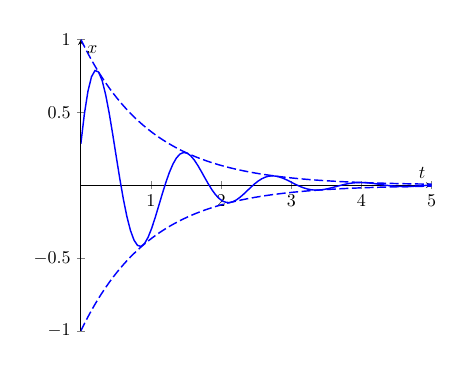
\begin{tikzpicture}[scale=0.65]
          \begin{axis}[
              domain=0:5,
              samples=100,
              axis lines=middle,
              xlabel=$t$,
              ylabel=$x$
            ]
            \addplot[blue, thick, dash pattern=on 5pt off 2pt] {e^(-x)};
            \addplot[blue, thick, dash pattern=on 5pt off 2pt] {-e^(-x)};
            \addplot[blue, thick] {e^(-x)*cos(deg(5*x + 5))};
          \end{axis}
        \end{tikzpicture}
        \caption{Hàm \(e^{-t} \cos{\left(5t + 5 \right)}\)}
    \end{figure}
\end{frame}
\begin{frame}{Trường hợp 2: \(\Delta > 0\)}
    Ta giải \(\lambda\)
    \begin{equation*}
        \lambda_{1,2} =  - \gamma \pm  \sqrt{\gamma^2 - \omega^2}.
    \end{equation*}    
    Nghiệm tổng quát:
    \begin{equation}
    \begin{array}{cl}
    x &= A e^{\lambda_1 t} + B e^{\lambda_2 t} \\
    &= e^{-\gamma t} \left(A e^{\sqrt{\gamma^2 - \omega^2} \ t} + B e^{- \sqrt{\gamma^2 - \omega^2} \ t} \right).
    \end{array}
    \label{eq:2.2_11}
    \end{equation}
\end{frame}
\begin{frame}{Trường hợp 2: \(\Delta > 0\)}
\begin{figure}[!htb]
    \centering
    \begin{tikzpicture}[scale=0.8]
      \begin{axis}[
          domain=0:2,
          samples=100,
          axis lines=middle,
          xlabel=$t$,
          ylabel=$x$
        ]
        \addplot[blue, thick] {20*e^(-(5-2)*x) +10*e^(-(5+2)*x};
      \end{axis}
    \end{tikzpicture}
    \caption{Hàm \(20 e^{-(5-2)t} + 10 e^{-(5+2)t}\)}
\end{figure}
\end{frame}
\begin{frame}{Trường hợp 3: \(\Delta = 0\)}
    Ta giải \(\lambda\)
    \begin{equation*}
        \lambda =  - \gamma.
    \end{equation*} 
    Nghiệm tổng quát
    \begin{equation}
        x = e^{-\gamma t} \left(A + Bt \right).
        \label{eq:2.2_12}
    \end{equation}
    \begin{figure}[!htb]
    \centering
    \begin{tikzpicture}[scale=0.57]
      \begin{axis}[
          domain=0:2,
          samples=100,
          axis lines=middle,
          xlabel=$t$,
          ylabel=$x$
        ]
        \addplot[blue, thick] {e^(-5*x)*(20 + 10*x)};
      \end{axis}
    \end{tikzpicture}
    \caption{Hàm \(e^{-5t} \left(20 + 10t\right)\)}
    \end{figure}
\end{frame}
\begin{frame}{Tổng kết}
    Với \(\alpha, \beta, \gamma \in \mathbf{R}\). Xét phương trình đặc trưng
    \begin{equation*}
        \alpha \lambda^2 + \beta \lambda + \gamma = 0.
    \end{equation*}
    \begin{equation*}
        \begin{array}{|l|c|}
        \hline
        \text{Trường hợp} & \text{Nghiệm} \\ 
        \hline
        \begin{array}{l}
        \Delta < 0 \\
        \lambda = a + ib
        \end{array}
        & x = C e^{-at} \cos(bt + \varphi) \\
        \hline
        \begin{array}{l}
        \Delta > 0 \\
        \lambda = \lambda_{1,2}
        \end{array}
        & x = Ae^{\lambda_1 t} + B e^{\lambda_2 t} \\
        \hline
        \begin{array}{l}
        \Delta = 0 \\
        \lambda = a
        \end{array}
        & x = e^{at} (A + Bt) \\
        \hline
        \end{array}
    \end{equation*}
\end{frame}